\documentclass{standalone}
\usepackage{pgfplots}
\pgfplotsset{compat=1.15}
\usepackage{mathrsfs}
\usetikzlibrary{arrows}
\newcommand{\degre}{\ensuremath{^\circ}}
\pagestyle{empty}

\tikzset{
  pics/handler/.style={perp},
  perp/.pic={                    
    \draw[black,line width=0.4pt](0,-0.05)--(0,.05);
  }
}

\begin{document}
\definecolor{zttcfw}{rgb}{0.5764705882352941,0.23529411764705882,0.9647058823529412}
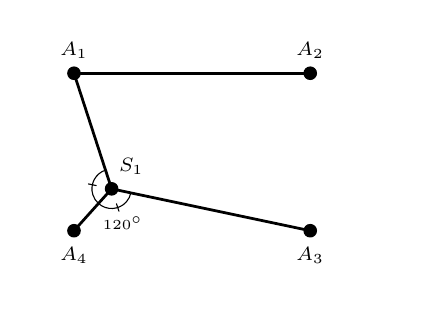
\begin{tikzpicture}[line cap=round,line join=round,>=triangle 45,x=1cm,y=1cm]
    \clip(-0.5882623610558796,-0.6382072431776696) rectangle (4.173633992296714,2.578644992402381);
    \draw[shift={(0.4778,0.532)},line width=0.4pt](0,0) -- (108.02886893898992:0.25) arc(108.02886893898992:228.0723452668876:0.25) pic[pos=.5,sloped]{perp};
    \draw[shift={(0.4778,0.532)},line width=0.4pt](0,0) -- (-131.92765473311243:0.25) arc(-131.92765473311243:-11.91063772611399:0.25) pic[pos=.5,sloped]{perp};
    \begin{scriptsize}
        \draw(0,2) node[circle,draw, fill=black, scale=0.6] (A1) [label={$A_1$}] {};
        \draw(3,2) node[circle,draw, fill=black, scale=0.6] (A2) [label={$A_2$}] {};
        \draw(3,0) node[circle,draw, fill=black, scale=0.6] (A3) [label={[yshift=-0.6cm]$A_3$}] {};
        \draw(0,0) node[circle,draw, fill=black, scale=0.6] (A4) [label={[yshift=-0.6cm]$A_4$}] {};
        \draw(0.4778,0.532) node[circle,draw,fill=black,scale=0.6] (S1) [label={[xshift=0.25cm]$S_1$}] {};

        % Edges
        \foreach \source/\target in {A1/S1, S1/A4, S1/A3, A1/A2} {
                \draw[black, line width=1pt] (\source) -- (\target);
            }

        \draw[color=black] (0.6203743000585789,0.1) node {\tiny{$120\textrm{\degre}$}};
    \end{scriptsize}
\end{tikzpicture}
\end{document}